\chapter{Algorithmen}\label{ch:algorithmen}
\wichtig{Forschungsfrage überlegen (Warum nicht DB zum Speichern von Spielerdaten)}

Verschiedene Theorien/Strategien von Speicher und Ladesysteme ausarbeiten und Zeiten messen (Mit Java und JSON hauptsächlich). Verschiedene Spielarten und Speichersysteme für diese ausarbeiten (Chunk Systeme machen vielleicht nicht überall Sinn, aber allgemein Daten aufteilen müsste gut sein)
%--------------------------------------------------------------------------
%--------------------------------------------------------------------------




%--------------------------------------------------------------------------
%--------------------------------------------------------------------------
\section{Speichersysteme}\label{sect:speichersysteme}
Theorie/Strategien von Speichersystemen und Bezug auf Arten von Videospiel-Daten.

Wichtiger unterschied zwischen ersten Speichern und das Speichern danach. Beim ersten Mal muss die Grundstruktur aufgebaut werden und auch mehr gespeichert werden.
%--------------------------------------------------------------------------


%--------------------------------------------------------------------------
\subsection{Daten in Videospielen}
Statische Daten (Maps, Texturen, etc.) und sich ändernde Daten (Spielerdaten und 
Daten zu dem Spielstand). Fokus dieser Arbeit sind nicht die statischen Daten!

Typen von Daten:\\
\begin{itemize}
    \item Statische Daten
    \begin{itemize}
        \item Grafikdaten
        \item Audiotechnische Daten
        \item Level- oder Kartendaten
    \end{itemize}
    \item Dynamische Daten
    \begin{itemize}
        \item Spielstand
        \item Benutzerdaten
    \end{itemize}
\end{itemize}
%--------------------------------------------------------------------------


%--------------------------------------------------------------------------
\subsection{Spielphasen}
\begin{figure}[htp]
    \centering
    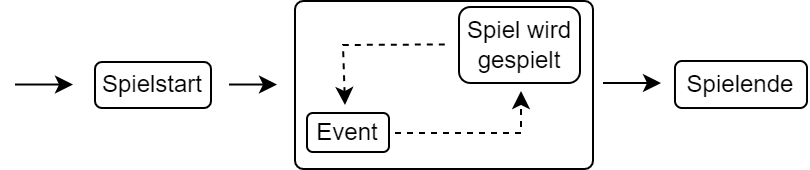
\includegraphics[width=0.8\textwidth]{images/Spielphasen.png}
    \caption{Phasen eines Spieles}
    \label{fig:spielphasen}
\end{figure}

\begin{itemize}
    \item Spielstart: Neues Spiel erstellen (und ggf. speichern) oder altes Spiel laden
    \item Event: Spielobjekt hat sich verändert oder wurde hinzugefügt/gelöscht
    \item Nach Event müssen ggf. Daten geladen werden (z.B. Spieler ist in einer neuen Zone)
    \item Spielende: Ggf. noch weitere Daten abspeichern
\end{itemize}

%--------------------------------------------------------------------------


%--------------------------------------------------------------------------
\subsection{Delta basierte Speicherung}
Das wichtigste um die Menge der gespeicherten Daten zu reduzieren, ist, dass man nur nur veränderte Daten speichert. Falls die zu speichernde Datenmenge nicht riesig ist, ist sowas auch nicht wirklich notwendig. Falls sich dafür entschieden wird, müssen folgende Events getracked werden:
\begin{itemize}
    \item Elemente werden hinzugefügt
    \item Elemente verändern sich
    \item Elemente werden gelöscht
\end{itemize}
%--------------------------------------------------------------------------


%--------------------------------------------------------------------------
\subsection{Aufteilung der Daten}
Chunking:
\begin{itemize}
    \item Hilfreich bei einer theoretisch unendlichen Welt
    \item Aufteilung der Mengen an Daten unter den Chunks
    \item Datengröße kann sich stark verändern, Chunk System muss sich anpassen
    \item Wenn Daten zu viele werden mehr Chunks
    \item Wenn Daten zu wenig werden weniger Chunks
    \item Chunk System nach Area, damit Laden effizienter läuft 
    (Nur Chunks mit seinen Elementen laden, wenn dieser in Nähe ist)
\end{itemize}

Szenen/Räume:
\begin{itemize}
    \item Falls die Spielwelt aus mehreren Szenen/Räumen besteht, Daten in diesen aufteilen
    \item Falls Szenen/Räume zu groß sind ggf. in Sektoren aufteilen
\end{itemize}
%--------------------------------------------------------------------------


%--------------------------------------------------------------------------
\subsection{Serialisieren}
\url{https://en.wikipedia.org/wiki/Comparison_of_data-serialization_formats}

Serialisierung ist der Prozess, bei dem der Zustand eine Objekts in ein Medium abgespeichert werden kann. Deserializierung ist der Gegenprozess, der den Zustand wieder zu einem Objekten formatiert. \wichtig{Beispiele zu jeder Serialisierung zeigen.\\
}\url{https://www.codeguru.com/csharp/c-sharp-serialization}

JSON:
\begin{itemize}
    \item JavaScript Object Notation
    \item Lesbarer Code
    \item Unterstützt nur String, Boolean, Number, Array, Object, null
    \item Wird für APIs, Konfigurations-Dateien und als Datenbank-Speicher verwendet 
\end{itemize}
\url{https://www.mongodb.com/json-and-bson}

Arten damit zu arbeiten:
\begin{itemize}
    \item Streaming API
    \item Tree Model
    \item Data Binding
\end{itemize}
\url{https://www.tutorialspoint.com/jackson/jackson_overview.htm}

BSON:
\begin{itemize}
    \item Binary JSON
    \item Kodiert JSON-Typen und speichert deren Länge (wodurch das Durchqueren der Daten schneller als bei JSON läuft)
    \item Nicht menschlich lesbar wie JSON
    \item Unterstützt mehr Typen
\end{itemize}
\url{https://www.mongodb.com/json-and-bson}

JSONH: (\url{https://stackoverflow.com/questions/11160941/is-it-worth-the-effort-to-try-to-reduce-json-size})



Binäre Serialisierung:
\begin{itemize}
    \item Konvertierung von Objekt zu Stream von Bytes
    \item Nicht leserlich für Menschen
\end{itemize}
\url{https://learn.microsoft.com/en-us/previous-versions/dotnet/fundamentals/serialization/binary/binary-serialization}
%--------------------------------------------------------------------------


%--------------------------------------------------------------------------
\subsection{Komprimierung der Daten}
Zippen der Daten:
\begin{itemize}
    \item Viel zippen vs. kleine Dateien (Kleine Chunks)
    \item Bringt lokales Zippen überhaupt was oder nur wenn man mit Server arbeitet?
\end{itemize}

Weitere Ideen:
\begin{itemize}
    \item Kürzere property Namen
    \item Null Werte ausschließen
    \item Vectoren in einem String (z.B. "1,2,3" für x=1, y=2, z=3)
\end{itemize}
%--------------------------------------------------------------------------


%--------------------------------------------------------------------------
\subsection{Schreibprozesse reduzieren}
Das Schreiben in den normalen Speicher ist zeitintensiv. Deshalb sollte möglichst wenig Daten auf die Festplatte geschrieben werden. Eine Möglichkeit ist es, die veränderungen über eine Liste im Arbeitsspeicher zu speichern und bei Programmterminierung diese Liste abzuspeichern. Dies ist aber riskant, da Daten verloren gegangen werden können bei frühzeitigen Löschen. Alternativ kann man diese Liste auf dem Festplattenspeicher führen und beim Laden des Spieles abarbeiten und dann leeren.
%--------------------------------------------------------------------------
%--------------------------------------------------------------------------




%--------------------------------------------------------------------------
%--------------------------------------------------------------------------
\section{Ladesysteme}\label{sect:ladesysteme}
Theorie vom Laden der Spieldaten
%--------------------------------------------------------------------------


%--------------------------------------------------------------------------
\subsection{Nearby Loading}
Nur die Daten laden, die in der Nähe vom Spieler sind (über Render-Distance). Ein Chunk-System (oder allgemein gute Aufteilung der Daten) dafür sehr vorteilhaft für effizienteres Laden, statt durch alle Elemente immer zu iterieren.
%--------------------------------------------------------------------------


%--------------------------------------------------------------------------
\subsection{Lazy Loading}
Prozedulares Laden der Daten (nicht alles auf einmal laden, sondern erst mal nur das nötigste und dann Stück für Stück den Rest nachladen). 
%--------------------------------------------------------------------------


%--------------------------------------------------------------------------
\subsection{Leseprozesse reduzieren}
\wichtig{Gibt vielleicht hier was zu schreiben}
%--------------------------------------------------------------------------
%--------------------------------------------------------------------------




%--------------------------------------------------------------------------
%--------------------------------------------------------------------------
\section{Strategien}
Aus den Strategien der vorherigen sections verschiedene Speicher- und Ladesysteme aufstellen und deren Effizienz auswerten.

\subsection{Allgemeines Speicher- und Ladesystem}
Allgemeines Speicher- und Ladesystems (manche Schritte optional)
\begin{figure}[htp]
    \centering
    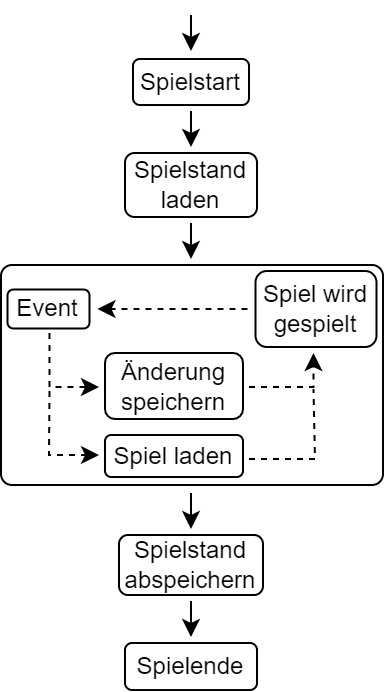
\includegraphics[width=0.36\textwidth]{images/Speichersystem.png}
    \caption{Phasen eines allgemeinen Speicher- und Ladesystems}
    \label{fig:speicherphasen}
\end{figure}

\begin{itemize}
    \item Spielstand laden kann alles auf einmal oder nur teile geladen werden (siehe mehr im Kapitel \ref{sect:ladesysteme})
    \item Je nach Speichersystem müssen hier teilweise noch die gespeicherten Daten überarbeitet werden
    \item Je nach Speichersystem können die Events die in "Änderung speichern" behandelt werden in zwei Kategorien unterteilt werden:
    \begin{enumerate}
        \item Ein Spielobjekt wurde hinzugefügt/geändert
        \item Ein Spielobjekt wurde gelöscht
    \end{enumerate}
    \item Spiel laden nach Events, wenn der Spieler sich z.B. in neuen Bereichen der Map befindet, die noch geladen werden müssen (mehr dazu in \ref{sect:ladesysteme})
    \item Spielstand am Ende abspeichern, vor Spielende optional (je nach Speichersystem notwendig)
\end{itemize}
%--------------------------------------------------------------------------


%--------------------------------------------------------------------------
\subsection{Chunk-basiertes System}
Chunk-basiertes System, welches Daten in Chunks verpackt:
\begin{figure}[htp]
    \centering
    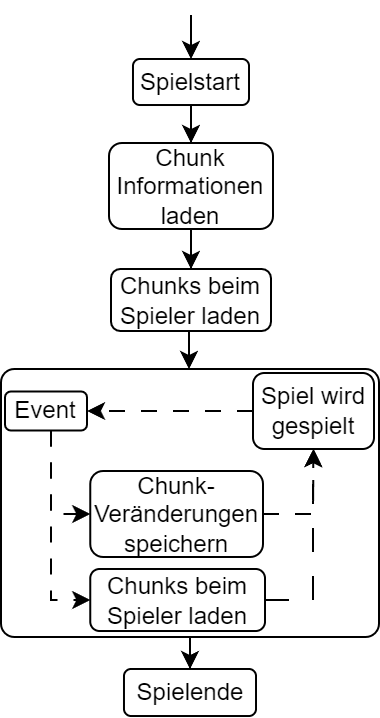
\includegraphics[width=0.36\textwidth]{images/Chunkbasiert.png}
    \caption{Chunk-basiertes System}
    \label{fig:chunkBasedSystem}
\end{figure}

Wobei ein Chunk aus folgenden Variablen besteht:
\begin{figure}[htp]
    \centering
    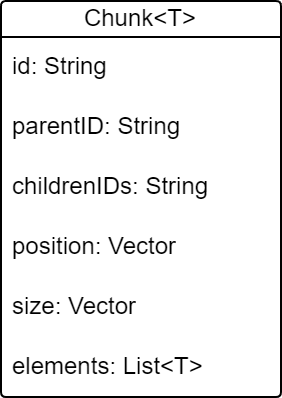
\includegraphics[width=0.28\textwidth]{images/Chunk.png}
    \caption{Chunk Klasse}
    \label{fig:chunkClass}
\end{figure}

\begin{itemize}
    \item Chunks haben Position und Größe
    \item Dynamische oder statische Chunk Größe (Entweder alle Chunks feste Größe, oder sie passen sich an Datenmenge an)
    \item Chunks speichern Objekte, die in deren Bereich sind
    \item ParentID und ChildrenIDs sind optional
\end{itemize}

Informationen zu dem System:

\begin{itemize}
    \item Objekte von Chunks in der Nähe des Spielers laden
    \begin{itemize}
        \item Allgemein werden Objekte eines Chunks erst dann laden, wenn es nötig ist (Z.B. Spieler in der Nähe); sowohl am Anfang, als auch während des Spieles
    \end{itemize}
    \item Chunk Veränderungen speichern bei statischer Chunkgröße:
    \begin{itemize}
        \item Daten zu Chunkinhalt komplett neu speichern bei update/added/removed Objekt Event
    \end{itemize}
    \item Chunk Veränderungen speichern bei dynamischer Chunkgröße:
    \begin{itemize}
        \item Daten zu Chunkinhalt komplett neu speichern bei update/added Objekt Event 
        \item Chunkgröße bei added/removed Objekt Event überprüfen
        \item Chunkdaten komplett vom Speicher löschen, wenn dieser im Spiel gelöscht wird (beim Joinen mit benachbarten Chunks)
        \item Chunkdaten updaten und hinzufügen, wenn ein Chunk auf weiter Child-Chunks gesplitted wird
    \end{itemize}
\end{itemize}

Alternative des Chunk-basierten Systems, um weniger Schreibprozesse auf dem lokalen Speicher zu haben:

\begin{figure}[htp]
    \centering
    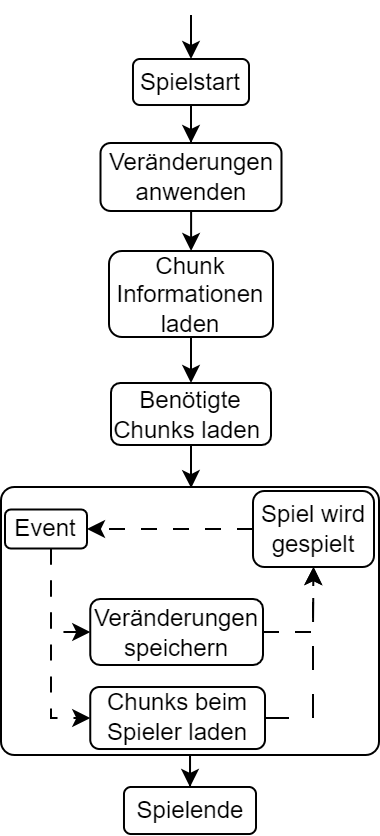
\includegraphics[width=0.36\textwidth]{images/Chunkbasiert2.png}
    \caption{Alternative zu dem Chunk-basierten System}
    \label{fig:altchunkBasedSystem}
\end{figure}

\begin{figure}[htp]
    \centering
    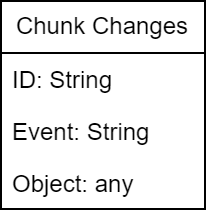
\includegraphics[width=0.25\textwidth]{images/Changes.png}
    \caption{Speichern von Veränderungen}
    \label{fig:changesClass}
\end{figure}

\begin{itemize}
    \item Veränderungen anwenden:
    \begin{itemize}
        \item Liste von Veränderungen des letzten Spielstandes werden lokal gespeichert (zum Beispiel als Objekte wie \ref{fig:changesClass} in JSON)
        \item Verschiedene Events = Unterschiedlich was Object ist
        \item Liste von oben nach unten abarbeiten, da erste Einträge die ältesten sind 
        \item Objekte aus Liste zu Chunk hinzufügen/updaten oder (bei dynamischer Chunkgröße) Chunks die nicht mehr gebraucht werden löschen
        \item Liste leeren
    \end{itemize}
    \item Nearby loading von Chunks wie beim anderen Chunk-basierten System
    \item Chunk-Veränderung speichern:
    \begin{itemize}
        \item Hinzugefügte/Veränderte/Gelöschte Objekte in Change Liste (im Arbeitsspeicher) speichern
        \item Entweder direkt in lokaler Change List Datei ans Ende hinzufügen oder erst bei Spielende (sehr riskant, falls Spiel ungewollt terminiert)
        \item Bei dynamischer Chunkgröße speichern wenn Chunks gelöscht/hinzugefügt wurden
    \end{itemize}
\end{itemize}
%--------------------------------------------------------------------------


%--------------------------------------------------------------------------
\subsection{Auswertung}
Auswertung der Strategien mit Daten/einfaches Spielkonzept mit Java und JSON testen:
\begin{itemize}
    \item Spieler (HP, LVL, Ausrüstung, Position, Rotation, ...)
    \item Gegner (HP, LVL, Ausrüstung, Position, Rotation, ...)
    \item Ausrüstung (Beschreibung/ID, Verteidigung, Angriff)
    \item Hindernisse (Beschreibung/ID, Position, Rotation)
    \item Items (Beschreibung/ID, Position, Rotation)
\end{itemize}

Klassendiagramm zeigen, um Daten des Spieles zu visualisieren. Testen der Effizienz mit JMH (Erklären was JMH ist und warum das gut dafür ist)

Zu beachtende Faktoren:
\begin{itemize}
    \item Chunk size
    \item Veränderungen
\end{itemize}